\chapter{Aprendizado de máquina e modulação do comportamento humano}

\begin{flushright}
\emph{Carla Oliveira}
\end{flushright}

As Tecnologias da Informação e Comunicação (TICs) permitiram a criação
de dispositivos tecnológicos capazes de minerar, analisar e agrupar
dados comportamentais e estruturá-los em uma base de dados para o
desenvolvimento de tudo que diz respeito à subjetividade e à emoção.
Segundo Cavalheiro e Brandão (2017) ``os fluxos de desejo são captados''
por essas ferramentas e direcionados de modo distribuído pelos meios de
comunicação, fazendo prevalecer ``os interesses de poucos, mas dando a
impressão de que é o desejo de muitos'' (p. 98).

Técnicas de persuasão utilizadas ao longo da história ganham outras
formas com esse novo cenário tecnológico. Algoritmos de Aprendizado de
Máquina são utilizados para impulsionar ideias, notícias e campanhas
publicitárias. Essas técnicas, que são utilizadas pela publicidade e
pelo marketing, também passaram a ser consideradas para ``influenciar a
opinião pública'' (Cavalheiro e Brandão, 2017, 89).

Inteligência Artificial (IA) e Aprendizado de Máquina são as
\emph{buzzwords} do momento, ou seja, ``palavras barulhentas'', e esse
barulho está ocorrendo não só na academia, mas principalmente no
mercado. De acordo Sugomori (2016) empresas de tecnologia, como Google e
Facebook, estão cada vez mais adquirindo \emph{startups} de IA. Em 2014,
foi anunciado que o Google comprou a \emph{Deep Mind} (Haas, 2014). Já
em 2018, foi a vez do Facebook investir US\$ 30 milhões na aquisição da
\emph{Bloomsbury}, especializada em processamento de linguagem natural
(Borini, 2018).

Para o pesquisador Pedro Domingos (2017), a ``Revolução Industrial
automatizou o trabalho manual e a Revolução da Informação fez o mesmo
com o trabalho mental''. Assim como a ``Internet'' e o ``computador
pessoal'', o Aprendizado de Máquina irá gerar grandes ``mudanças
econômicas e sociais'' (p. 33). Mas, o que é Aprendizado de Máquina?

De acordo com Domingos (2017) \emph{Machine Learning,} também conhecido
como Aprendizado de Máquina, é um subconjunto da Inteligência
Artificial. O Aprendizado de Máquina ``é uma tecnologia que constrói a
si própria''. Ao contrário dos algoritmos tradicionais, os algoritmos de
Aprendizado ``são artefatos que projetam outros artefatos'' (p. 16).
``Os aprendizes transformam dados em algoritmos'' e neste caso quanto
mais dados (\emph{Big Data}) melhor (p. 17). Com o Aprendizado de
Máquina pode-se dizer que os computadores são capazes de criar seus
próprios algoritmos (Ibid.).

Para Domingos (2017), a essência do Aprendizado de Máquina é a previsão
de desejos, comportamentos e de como o mundo poderá ser alterado. Para
ele, o Aprendizado de Máquina está ``recriando a ciência, a tecnologia,
os negócios, a política e a guerra'' (p. 16). O pesquisador alerta para
o fato de que não podemos controlar aquilo que não compreendemos. Por
isso é importante entender o que é Aprendizado de Máquina e como esse
tipo de tecnologia está sendo utilizado.

Este texto visa definir o que é Aprendizado de Máquina e como esta
tecnologia pode ser utilizada como dispositivo de modulação. Para tanto,
apresenta a evolução da IA até o surgimento do Aprendizado de Máquina.
Em seguida, mostra a definição de sociedade de controle e modulação.
Para estabelecer uma relação entre modulação e Aprendizado de Máquina
considera algumas pesquisas utilizando psicometria, rastros digitais dos
usuários e Aprendizado de Máquina, serviços do Facebook e seus
algoritmos de \emph{Machine Learning} e a utilização de Aprendizado de
Máquina para fins políticos nas eleições de Barack Obama e Donald Trump.

\section{Inteligência Artificial e sua evolução}

O embrião da Inteligência Artificial surgiu em 1943, com o artigo
``\emph{A logical calculus of the ideas immanent in nervous activity}''
(McCulloch e Pitts, 1943), escrito pelo Psiquiatra Warren S. McCulloch e
pelo Cientista Cognitivo, Walter Pitts. Este artigo visou estabelecer
uma analogia entre as células nervosas e o processo eletrônico. Este
artigo pode ser considerado como o primeiro modelo de Redes Neurais
Artificiais.

Em 1950, Alan Turing, um dos pais da Ciência da Computação e da
Inteligência Artificial, publicou o artigo ``\emph{Computing Machinery
and Intelligence}'' (Turing, 1950), na revista inglesa, \emph{Mind}.
Neste artigo, foi proposto o seguinte questionamento: ``As máquinas
podem pensar?'' Devido à complexidade dos termos ``Máquina'' e
``Pensar'', Turing procurou a resposta para esta dúvida por meio de um
jogo, o qual batizou de ``Jogo da Imitação'' (Turing, 1950). Mais tarde
esse jogo ficou conhecido como ``Teste de Turing''.

O termo Inteligência Artificial (IA) foi apresentado pela primeira vez
pelo cientista da computação, John McCarthy, na 2ª Conferência de
Dartmouth, em 1956 (Júnior e Lima, 2010). Pesquisas relacionadas a IA
vêm sendo desenvolvidas há décadas.

O primeiro \emph{boom} da IA surgiu no final dos anos 50 com programas
de busca baseados em regras fixas. Embora os métodos de busca tivessem
grande sucesso em campos específicos como o Xadrez e o Shogi (versão
japonesa do jogo de xadrez) estava longe de atingir a IA (Sugomori,
2016).

O segundo \emph{boom} da IA ocorreu nos anos 80 com o movimento
denominado Representação do Conhecimento (Sugomori, 2016). Vários
métodos de Representação do Conhecimento foram desenvolvidos para
projetar conhecimento em uma máquina. Um exemplo deles é o Cyc\footnote{http://www.cyc.com}.
Este sistema foi criado em 1984, por Douglas Lenat, pesquisador na área
de Inteligência Artificial (Domingos, 2017). Trata-se de um enorme banco
de dados suportado por tecnologias semânticas que combina uma base de
conhecimento comum com mecanismo de inferência.

No decorrer do tempo, um novo método denominado \emph{Machine Learning}
(Aprendizado de Máquina) surgiu e com ele a possibilidade de atingir a
IA se tornou mais factível. O \emph{Machine Learning} está intimamente
relacionado à mineração de dados e \emph{Big Data}. De acordo com
Sugomori (2016), este novo método é uma ferramenta potente em comparação
às abordagens anteriores que simplesmente tinham como base o
conhecimento fornecido previamente por um ser humano.

Antes do \emph{Machine Learning,} uma máquina só fornecia resposta com
base nos dados e regras fixas que já haviam sido inseridos. Neste
cenário a máquina fornecia rapidamente respostas para uma pergunta
previamente conhecida, mas literalmente travava quando surgiam questões
desconhecidas.

No \emph{Machine Learning}, a máquina pode lidar com questões
desconhecidas com base no conhecimento que aprendeu anteriormente. Neste
caso, pode-se afirmar que o \emph{Machine Learning} é um método de
reconhecimento de padrões. Sugomori (2016) explica que, no \emph{Machine
Learning,} a máquina utiliza uma quantidade gigantesca de dados de
treinamento, substituindo perguntas complexas por perguntas do tipo
``sim'' ou ``não'' (0 ou 1) e descobre a regularidade com que os dados
são marcados com ``sim'' e com ``não''. Em suma, esse sistema pode dar
uma resposta reconhecendo e classificando os padrões a partir dos dados
fornecidos e, em seguida, classificando esses dados no padrão apropriado
(previsão). Dessa forma, quando a máquina se depara com dados
desconhecidos numa pergunta é capaz de fazer uma previsão e fornecer uma
resposta.

O \emph{Machine Learning} é um método que possibilita que uma máquina
possa processar esse reconhecimento de padrões de forma autônoma sem
nenhuma interferência humana. Este padrão de classificação é baseado em
uma fórmula numérica chamada de modelo estatístico probabilístico. Esta
abordagem tem sido estudada com base em vários modelos matemáticos
(Sugomori, 2016). No processo de treinamento, os parâmetros de um modelo
são ajustados, e, uma vez concluído o aprendizado, são atualizados com
esses novos parâmetros. A máquina então categoriza dados desconhecidos
no padrão que se ajusta melhor aos parâmetros aprendidos.

Com o \emph{Machine Learning,} as máquinas tornaram-se capazes de
processar dados e fornecer respostas que os humanos não são capazes de
fazer. Segundo Sugomori (2016), o conceito de \emph{Machine Learning} em
si vem de longa data, contudo pesquisadores não tiveram condições de
provar a utilidade desse método anteriormente devido à tecnologia da
época não suportar o processamento de um alto volume de dados e também
pela própria falta de dados.

Atualmente, esse problema foi solucionado. Com a enorme quantidade de
dados e códigos-fonte abertos, os pesquisadores puderam experimentar os
algoritmos usando todo esse arsenal. Graças à alta capacidade de
processamento dos computadores atuais, várias opções de algoritmos e
dados, o \emph{Machine Learning} foi cada vez mais aperfeiçoado e com
isso surgiu o terceiro boom da IA.

O \emph{Machine Learnin}g sem dúvida é um poderoso método quando se
trata da mineração de dados e foi o pontapé inicial para o terceiro
\emph{boom} da IA. Contudo, não foi suficiente para alcançar
definitivamente o conceito de IA. Mas isso não significa que essa
odisseia chegou ao fim. O terceiro boom está apenas começando e uma nova
onda está a caminho com o \emph{Deep Learning}. Com o advento deste novo
método (pelo menos nas áreas de reconhecimento de imagem e voz), uma
máquina tornou-se capaz de decidir a partir dos dados disponibilizados e
escolher os melhores dados sem necessidade de manipulação humana.

O \emph{Deep Learning} é apenas o primeiro passo para uma máquina obter
conhecimento de forma semelhante aos humanos. É difícil prever qual a
próxima inovação. De acordo com a lei de Moore, o número de transistores
dobra a cada 18 meses, ou seja, um ano e meio (Sugomori, 2016). De
acordo com Sugomori, se essa técnica continuar nesse ritmo, o número de
transistores ultrapassará dez bilhões, número esse que corresponde à
quantidade de células no cérebro humano. Considerando a lei de Moore, em
2045, ele acredita que chegaremos a um ponto crítico chamado
``Singularidade Técnica'' (Sugomori, 2016).

O termo ``Singularidade Técnica'' foi criado pelo cientista Vernor
Vinge, que discorre sobre este tema no artigo ``\emph{The Coming
Technological Singularity: How to Survive in the Post-Human Era}'',
(Vinge, 1993). Resumidamente, Vinge descreve quatro itens tecnológicos
que podem levar à ``Singularidade Técnica'' e à superação dos homens
pelas máquinas: 1) A velocidade com que os computadores são
aperfeiçoados e a evolução da Inteligência Artificial; 2) As redes de
computadores se tornarem autoconscientes; 3) As interfaces homem-máquina
se tornarem tão complexas que produziriam um estágio evolutivo do homem
e 4) A ampliação da inteligência humana natural através de melhores
técnicas da ciência biológica (Ibid.).

Em contrapartida, o filósofo John Searle, em seu artigo ``\emph{Minds,
brains and programs}'', (Searle, 1980), critica a Inteligência
Artificial a qual dividiu em Inteligência Artificial Forte e
Inteligência Artificial Fraca. Para o filósofo, Inteligência Artificial
Forte é uma IA capaz de simular totalmente a inteligência humana. Já a
Inteligência Artificial Fraca se associa a métodos específicos, que dão
conta de funções especializadas da inteligência humana.

De acordo com Amorim (2014), o pensamento de Searle teve por objetivo
mostrar que não é possível replicar totalmente a mente humana utilizando
a lógica binária (0 e 1) dos softwares (programas de computador). Para
comprovar essa teoria, Searle apresentou o argumento do ``Quarto
Chinês'' como crítica à Inteligência Artificial Forte e ao Teste de
Turing. Este argumento teve por finalidade elucidar a impossibilidade de
duplicação da inteligência humana por meio de algoritmos e para isso
Searle fez uma analogia entre uma pessoa dentro de um quarto chinês,
onde o quarto é o computador e a pessoa o programa. Neste quarto
(computador) a pessoa (programa) não compreende o significado dos
símbolos em chinês e mesmo assim consegue responder perguntas em chinês
com base em regras definidas (Amorim, 2014).

Atualmente há muitos anúncios de produtos, como sistemas de recomendação
e, assistentes virtuais, dizendo que utilizam IA. Para Sugomori (2016),
esse tipo de anúncio não é correto, pois a palavra Inteligência
Artificial é usada como um conceito mais abrangente. Ele explica que as
pesquisas e técnicas acumuladas no passado alcançaram apenas algumas
ramificações da IA e as pessoas utilizam este termo de forma errada para
designar essas ramificações.

Para Biddle (2018) ``o termo Inteligência Artificial foi banalizado''
como tantas outras \emph{buzzrwords} do ``mundo digital''. Ele considera
IA como um conceito abrangente que possui subconjuntos, como o
Aprendizado de Máquina, que permite aos computadores aprenderem sozinhos
e se tornarem mais eficientes numa enorme variedade de aplicações, como
o reconhecimento facial, a detecção de fraudes financeiras, entre outras
(Biddle, 2018, Online).

De acordo com Domingos (2017) o Aprendizado de Máquina é conhecido por
vários termos: ``reconhecimento de padrões, modelagem estatística,
mineração de dados, descoberta de conhecimento, análise preditiva,
ciência de dados, sistemas adaptativos'', entre outros (p. 31). Ele
alerta para o fato de o \emph{Machine Learning} ser confundido com
Inteligência Artificial e esclarece essa confusão ao explicar que
\emph{Machine Learning} é um subconjunto da Inteligência Artificial. Ou
seja, a IA deve ser considerada como um grande guarda-chuva para
diversos métodos. Resumidamente \emph{Machine Learning} é um subconjunto
da IA e \emph{Deep Learning} um subconjunto do \emph{Machine Learning}.

Como o Aprendizado de Máquina pode ser utilizado como dispositivo de
controle e modulação do comportamento humano? O próximo item traz
conceitos e exemplos que ajudam a elucidar isso.

\section{Aprendizado de máquina e modulação do comportamento humano}

Em seu \emph{post-scriptum} sobre as sociedades de controle, Deleuze
(1992) descreve que Foucault situou as sociedades disciplinares nos
séculos XVIII e XIX e seu apogeu no século XX. A grande marca desse tipo
de sociedade são os meios de confinamento, onde os indivíduos passam de
um meio fechado para outro, de casa para a escola, da escola para a
fábrica, além dos hospitais e presídios. De acordo com Deleuze (1992),
Foucault fez uma análise desses meios de confinamento, especialmente na
fábrica, onde era preciso compor no espaço-tempo uma força produtiva. No
entanto, Foucault sabia da brevidade desse modelo e do surgimento de um
novo tipo de sociedade.

A era da disciplina deu lugar a uma nova era que Deleuze denominou era
do controle. Lazzarato (2006) mostra algumas características das
sociedades disciplinares para facilitar a compreensão dessa nova era. De
acordo com ele, as sociedades disciplinares são caracterizadas pelo
poder disciplinar e biopolítico. As técnicas disciplinares transformam
os corpos, enquanto as técnicas biopolíticas são aplicadas na massa, em
processos como o nascimento, a morte, a reprodução e a doença. A
disciplina conhece o corpo e o indivíduo, enquanto o biopoder foca na
população e na gestão da vida.

Para Lazzarato (2006), as sociedades de controle criaram tecnologias e
processos de subjetivação que são bem diferentes das tecnologias e
processos das sociedades disciplinares. Com o intuito de descrever a
sociedade de controle, ele recorre a três características desse novo
tipo de tecnologia de poder: 1) a emergência da cooperação entre
cérebros e seu funcionamento por fluxos e redes; 2) dispositivos
tecnológicos que agem à distância e amplificam a potência de ação, tais
como a televisão e a Internet, e 3) a formação dos públicos por meio dos
processos de subjetivação e sujeição (Lazzarato, 2006, 76).

Lazzarato (2006) considera que ``a captura, o controle e a regulação da
ação à distância das mentes entre si se faz por meio da modulação dos
fluxos de desejos, crenças e das forças (memória e atenção) que circulam
entre os cérebros'' (p. 84). Para ele, ``a memória, a atenção e as
relações que elas atualizam tornam-se forças sociais e econômicas que
precisam ser capturadas para que possam ser controladas e exploradas''
(p. 84).

Em relação à cooperação entre os cérebros, Lazzarato (2006) explica que
ela se expressa sob a forma de opinião pública, mediada pela tecnologia.
Para ele a ``Internet integra e distingue as diferentes transformações
da opinião pública, da percepção e da inteligência coletiva''. A divisão
da sociedade em públicos se sobressai da divisão religiosa, econômica,
estética, política, porém sem substituí-las (Lazzarato, 2006, 77-78).

Outra diferença entre as sociedades disciplinares e as sociedades de
controle citada por Lazzarato (2006), é que esta última investe na
memória mental e não no corpo. As ``disciplinas moldavam os corpos''
(p.86) construindo hábitos, já as sociedades de controle modulam os
cérebros criando hábitos na memória.

Para Deleuze (1992), os diferentes modos de controle, os
``controlatos'', são variações inseparáveis, formando um sistema cuja
linguagem é numérica. Os confinamentos são moldagens fixas, já os
controles são uma modulação que muda constantemente. Nas sociedades de
controle, ``o essencial não é mais uma assinatura'' e uma ``matricula''
como ocorria nas sociedades disciplinares, mas sim, uma ``cifra'' ou
senha. ``Os indivíduos tornaram-se dividuais e as massas tornaram-se
amostras, dados, mercados, bancos'' (Deleuze, 1992, 226).

A sociedade de controle exerce seu poder utilizando tecnologias de ação
e controle à distância que enviam imagens, som e informações por meio de
máquinas de modular. Este tipo de tecnologia são ``formas ultrarrápidas
de controle ao ar livre que substituem antigas disciplinas que operavam
em um sistema fechado''. (Deleuze, 1992, 224).

Mas afinal, o que é modulação como exercício de poder (LAZZARATO, 2006)?
``Nas sociedades de controle, as relações de poder se expressam pela
ação à distância de uma mente sobre outra, pela capacidade de afetar e
ser afetado dos cérebros, midiatizada e enriquecida pela tecnologia''
(p. 76). ``As instituições das sociedades de controle são assim
caracterizadas pelo emprego das tecnologias de ação à distância'' (p.
77). ``A captura, o controle e a regulação da ação a distância das
mentes entre si se faz através da modulação dos fluxos, de desejos, de
crenças, memória e atenção que as fazem circular entre os cérebros'' (p.
84). ``As máquinas de modular o tempo são dispositivos capazes de
intervir no acontecimento, na cooperação entre os cérebros, através da
modulação das forças envolvidas nessa cooperação, tornando-se assim a
condição necessária de todo processo de constituição de uma
subjetividade'' (p. 85-86).

Assim como é preciso compreender as diferenças entre as sociedades
disciplinares e as sociedades de controle, é necessário diferenciar os
dispositivos de manipulação dos dispositivos de modulação (Silveira,
2017). As empresas do ramo jornalístico podem ser consideradas como
dispositivos para expressão da ``prática dos jogos de verdade'', ou
seja, como dispositivos de manipulação. ``A verdade é em si poder. Uma
verdade é construída manipulando elementos da realidade, unindo em
determinado sentido os fatos, selecionando o que relatar e o que
desconsiderar ou omitir'' (Silveira, 2017, loc. 1229).

Foucault (2015) descreve que em nossa sociedade, a ``economia política''
da verdade tem cinco características: 1) a verdade é centrada na forma
do discurso científico e nas instituições que o produzem; 2) está
submetida a uma constante incitação econômica e política; 3) é objeto de
uma imensa difusão e de um imenso consumo; 4) é produzida e transmitida
sob o controle, não exclusivo, mas dominante, de alguns grandes
aparelhos políticos ou econômicos; 5) por fim, é objeto de debate
político e de confronto social (p. 52).

Na percepção de Silveira (2017), os dispositivos de modulação são
diferentes dos dispositivos de manipulação ou de criação de verdade por
meio do discurso. Para ele, os ``moduladores'' são
``actantes''\footnote{Actante é tudo aquilo que gera uma ação, que
  produz movimento e diferença, seja ele humano ou não-humano. O actante
  é o mediador, ou seja, é aquele que transforma, traduz, distorce e
  modifica o significado que ele supostamente transporta (Praude, 2015
  apud Latour, 2012; Latour, 2000).}, ``humanos'' e ``não humanos'' que
visam intermediar e facilitar o cotidiano das pessoas (loc. 1229).

Com a evolução da propaganda, uma máquina muito bem estruturada desses
actantes se desenvolveu, da qual o \emph{Google} e o \emph{Facebook} se
destacam: ``imensos bancos de dados'' (\emph{Big Data}) e softwares de
Aprendizado de Máquina que atuam como dispositivos de reconhecimento de
padrões, comportamentos e de marketing. Estes dispositivos ``reúnem,
selecionam e vendem milhões de dados sobre nossas aquisições, hábitos de
leitura, filmes favoritos, gostos, roupas, bem como o modo como passamos
nosso tempo livre'' (Lazzarato, 2014, 38). Esses dados configuram os
``dividuais'', ``amostras'' e ``dados'' definidos por Deleuse, cuja
finalidade é a modulação (Deleuse,1992, 226).

Essa ``megamáquina'' aos poucos foi diminuindo o ``número de operadores
humanos, não confiáveis'', e aumentando os ``agentes eletrônicos
confiáveis''. ``As novas máquinas sociais e técnicas'' e seus
dispositivos vão além da fábrica, elas se apoderaram do comportamento e
das ações das pessoas, não apenas no trabalho, mas também na vida
cotidiana (LAZZARATO, 2014, 34-35).

Para Silveira, a modulação do comportamento humano, é o principal
objetivo do mercado, quando este busca ferramentas para mineração e
análise de dados pessoais. Segundo ele, as técnicas de modulação não são
simplesmente a difusão de notícias e publicidade, mas a criação de
``situações sociais''. Os dispositivos de modulação são eficazes porque
atuam sobre nossa memória e atenção e, também porque na maioria das
vezes, são fundamentados com base na nossa subjetividade e emoção
(SILVEIRA, 2017, loc. 1228).

Silveira (2017) explica que após armazenar, minerar e analisar os dados,
as empresas definem amostras de perfis semelhantes que servem aos
dispositivos de modulação. A partir ``dos gostos, do temperamento, das
necessidades, das possibilidades financeiras, do nível educacional'',
entre outras categorias, as empresas oferecem ``soluções, produtos e
serviços'' para este grupo potencial de consumidores cujos dados foram
analisados (loc. 1285). Por isso, o sucesso da modulação requer uma
análise rigorosa das pessoas que serão moduladas.

No entanto, ``modular o que passará a ser imprescindível ou útil para o
cotidiano de uma pessoa ou grupo social é muito complexo'' (Silveira,
2017, loc. 1294). Está relacionado com a prática preditiva que depende
de tecnologias como \emph{Big Data}, Aprendizado de Máquina e estudos
das ciências cognitivas. De acordo, com Silveira, atualmente percebe-se
o uso cada vez maior das neurociências e da psicologia na composição das
equipes de marketing. A predição do que as pessoas estão interessadas em
saber pode gerar possibilidades de ``modular caminhos, restringir
escolhas e incentivar opções'' (Silveira, 2017, loc. 1294).

Michal Kosinski e seus artigos são ótimas fontes para entender o uso dos
dados pessoais e Aprendizado de Máquina para predição e modulação do
comportamento humano. Ele é psicólogo, cientista de dados e professor
\emph{na Stanford Graduate School of Business}. Possui doutorado em
psicologia, mestrado em psicometria e psicologia social. Kosinski
pesquisa os seres humanos utilizando os rastros digitais (\emph{Big
Data}) deixados em plataformas e dispositivos combinando conceitos de
psicometria, ciência social, psicologia, e Aprendizado de Máquina.

Durante o doutorado, Kosinski e outros colaboradores, criaram o
aplicativo \emph{MyPersonality}. Neste aplicativo foram disponibilizados
vários questionários psicométricos, com base nas perguntas do \emph{Big
Five}. O objetivo era que alguns amigos preenchessem os questionários,
mas para surpresa deles, ``milhões lhes revelaram suas crenças,
sentimentos e comportamentos''. Como resultado, eles se viram perante o
``maior banco de dados de personalidade da história'' (Guareschi, 2017,
173).

Avaliações psicométricas fazem parte de um ramo da psicologia denominado
psicometria que é uma área da psicologia que analisa e mensura
características psicológicas e a personalidade do individuo. Um dos
mecanismos utilizados é o \emph{Big Five} (cinco dimensões centrais da
personalidade dos seres humanos). Essas avalições foram compostas por
diferentes psicólogos, na década de 1980, por meio de uma análise
fatorial dos dados proporcionados pelas pessoas pesquisadas a partir de
``inventários de personalidade'' e de ``extensos questionários''. Todas
as informações foram sintetizadas em cinco principais fatores: abertura
ao novo, consciência, sociabilidade, extroversão e traços neuróticos
(Guareschi, 2017, 173).

De acordo com Kosinski et al (2013), a predição de características e
atributos individuais com base em testes psicométricos vem de longa
data. Atualmente, as atividades humanas e suas interações sociais são
mediadas por plataformas e dispositivos digitais. Essa crescente imersão
em ambientes digitais e a dependência dos dispositivos fizeram com que
os traços de comportamentos, comunicação, interações sociais, ou seja,
os rastros digitais das pessoas fossem facilmente registrados (Kosinski
et al, 2017).

Para Kosinski et al (2016), a disponibilidade desses rastros digitais,
juntamente com poder de computação e algoritmos de Aprendizado de
Máquina, oferece grandes oportunidades para a ciência social, pois
grandes volumes de dados facilitam a descoberta de padrões que podem não
estar disponíveis em amostras menores, além de contribuir para reduzir
erros de amostragem. Modelos preditivos baseados em pegadas digitais
(\emph{digital footprints}) também podem ser usados para desenvolver
ferramentas de diagnóstico e medidas psicométricas úteis para pesquisa e
prática psicológica. Além disso, abriram caminho para o surgimento da
ciência social computacional.

Kosinski et al (2013) alertam que as pessoas podem até optar por não
revelar certas informações sobre suas vidas, e mesmo assim essas
informações serem previstas com base em outros aspectos que elas expõem
por meio de seus rastros digitais. Este tipo de previsão pode ser
utilizado para melhorar produtos e serviços, mas de uma forma negativa,
podem levar a invasões de privacidade.

Em 2014, Kosinski e seus colaborados fizeram uma pesquisa para validar
se os julgamentos de personalidade feitos por um computador são mais
precisos do que os realizados por humanos. Esta pesquisa foi documentada
no artigo ``\emph{Computer-based personality judgments are more accurate
than those made byhumans}'', (Youyou et al, 2014). De acordo com os
pesquisadores, os resultados desse artigo mostraram que os modelos
baseados em computador são mais precisos que os humanos na tarefa de
julgamento da personalidade. Segundo Cadwalladr (2018), este artigo
serviu de inspiração para que Robert Mercer investisse na criação da
Cambridge Analytica.

Youyou et al (2014) concluíram neste estudo que ferramentas de avaliação
de personalidade automatizadas são precisas e de baixo custo e podem
afetar a sociedade das seguintes formas: mensagens de marketing podem
ser adaptadas às personalidades dos usuários; recrutadores podem
combinar melhor os candidatos com trabalhos tendo como base a
personalidade dos mesmos e produtos e serviços podem se ajustar para
corresponder melhor aos seus usuários (Youyou et al, 2014, 4).

Entretanto, Youyou et al (2014) destacam que o conhecimento a respeito
da personalidade das pessoas também pode ser utilizado para modulá-las e
influenciá-las. Por este motivo, as pessoas podem não aceitar esse tipo
tecnologia ao perceberem que o governo, redes sociais ou mecanismos de
busca podem predizer suas características pessoais com mais precisão do
que seus próprios familiares e amigos. Diante disso, os autores esperam
que desenvolvedores de tecnologia e formuladores de políticas considerem
esses desafios e se apoiem em leis de proteção dos dados.

Segundo Matza et al (2017), a comunicação de massa persuasiva é
utilizada por governos, marketing e partidos políticos e tem por
objetivo incentivar grupos de pessoas a acreditar e agir de acordo com o
ponto de vista do comunicador. Estudos mostram que, quando adaptada às
características e motivações psicológicas das pessoas, a comunicação de
massa persuasiva se mostra eficaz. Contudo, quando esses estudos são
realizados por meio de questionários, em laboratório, e com uma amostra
reduzida, a eficácia é limitada devido aos vieses de resposta e outras
razões que levam o comportamento das pessoas a diferir do apresentado em
laboratório. Diante desses fatos, é questionável se esses resultados
podem ser generalizados para a massa no mundo real.

Pesquisas recentes no campo das ciências sociais computacionais sugerem
que os perfis psicológicos das pessoas podem ser previstos com precisão
a partir dos rastros digitais que elas deixam. Para validar se a
segmentação psicológica traçada com base nos rastros digitais é eficaz
para persuasão de massa, Matza et al (2017) realizaram três
experimentos, com mais de 3,7 milhões de pessoas. O resultado comprovou
a eficácia do direcionamento psicológico no contexto da persuasão
digital em massa. A adaptação de apelos persuasivos aos perfis
psicológicos permitiu influenciar o comportamento e escolhas dos
participantes. O experimento foi medido com base nos cliques\footnote{Taxas
  de cliques (CTRs) são uma medida comum de marketing digital que
  quantifica o número de cliques em relação ao número de vezes que o
  anúncio foi mostrando.} e conversões\footnote{Taxa de conversão é uma
  métrica de marketing que reflete o número de conversões, como
  downloads de aplicativos ou compras em lojas on-line, em relação ao
  número de vezes que o anúncio foi exibido.} efetuados pelos
participantes. Contudo, apesar dos três experimentos terem sido
bem-sucedidos, Matza et al (2017) evidenciam pontos críticos que merecem
atenção.

O primeiro deles é que a eficácia da persuasão psicológica em larga
escala no ambiente digital depende muito da alta precisão na previsão
dos perfis psicológicos. A precisão é um item importante, pois quanto
menor a taxa de erro mais assertiva é a previsão. Mesmo que a previsão
utilize \emph{Big Data} e seja feita por Aprendizagem de Máquina, não
está livre de limitações, como a necessidade de calibrar e atualizar
constantemente o algoritmo. Matza et al (2017) dão o seguinte exemplo:
gostar de ``\emph{Game of Thrones}'' quando a série de TV foi lançada em
2011 poderia ser um indicador de introversão, contudo, a crescente
popularidade da série pode ter tornado isso menos previsível. Outro
ponto que pode afetar a precisão é que, apesar da avaliação psicológica
das impressões digitais permitir definir o perfil de um grande número de
pessoas sem o preenchimento de questionários, a maioria dos algoritmos
são desenvolvidas com base nesses questionários e podem absorver alguns
problemas dos mesmos.

Por fim, Matza et al (2017) chamam a atenção para o fato de que a
implementação da persuasão psicológica em massa, embora ofereça
oportunidades, também acarreta riscos e desafios éticos. Ela tanto pode
ser utilizada para ajudar as pessoas a tomar melhores decisões e aliviar
problemas sociais quanto para explorar pontos fracos ou modular as
pessoas a se comportarem de maneira que não são do interesse delas. Os
autores citam relatos da mídia alegando que a campanha presidencial dos
EUA, de 2016, usou perfis psicológicos de milhões de cidadãos dos EUA
para suprimir votos e mantê-los longe das eleições. Eles também
levantaram a questão da falta de legislação para proteção da privacidade
dos dados no ambiente digital. Embora eles tenham tido o cuidado de
realizar uma segmentação indireta mantendo o anonimato e privacidade
individual dos participantes, os experimentos também poderiam ser usados
para revelar traços íntimos dos indivíduos sem o consentimento dos
mesmos.

Ao ler os artigos de Michal Kosinski percebe-se que no início o
interesse era apenas incluir as pessoas analisadas em algumas dimensões
do \emph{Big Five}. Depois Kosinski e seus colaboradores passaram a
comparar os resultados com o que os pesquisados curtiam, compartilhavam
e postavam no Facebook e posteriormente passaram a cruzar esses dados
com os dados de outras plataformas digitais. Surgiu dessa forma a
possibilidade de traçar perfis segmentados e comparações entre esses
perfis (Guareschi, 2017).

Essa descoberta contribuiu para áreas como a da ``psicologia da
persuasão, publicidade, política e economia'', pois ``dependendo da
quantidade de pessoas investigadas nas redes sociais'' e dos rastros
digitais dessas pessoas em outras plataformas, é possível criar ``perfis
minuciosos e detalhados'' que podem ser utilizados para estudos de todo
o tipo, como para fins políticos, de publicidade, entre outros
(Guareschi, 2017, 173).

Isso mostra o poder que está em fazer uso de enormes quantidades de
dados (\emph{Big Data}). Não há nenhuma restrição tecnológica que impeça
os computadores de analisar milhões de dados sobre o comportamento das
pessoas e extrair tendências suficientes para que se possa conhecer o
que essas pessoas pensam, acreditam, gostam, quais valores defendem e as
motivações que as movem. Não há dúvidas de que ``sempre haverá pessoas
que discordam de determinadas opiniões ou valores'', ``mas isso não tem
importância para quem sabe que seus anúncios vão atingir milhões
influenciados por essas mensagens'' (Guareschi, 2017, 175).

Atualmente, podemos considerar a postagem e a curtida como sendo
semelhante ao ato de responder ao ``questionário ou uma entrevista
dirigida''. Outras opções de ``oferecimento gratuito de informação'' são
os compartilhamentos e comentários. À medida que usuários postam
mensagens no Facebook, ou em outras redes sociais, sem que tenham
consciência, um algoritmo de Aprendizado de Máquina vai sendo
constantemente construído e atualizado com base nesse imenso banco de
dados ``livremente oferecido''. (Guareschi, 2017, 176).

O \emph{The Intercept}, site lançado em 2014, pelo jornalista Glenn
Greenwald, a cineasta Laura Poitras e o pesquisador Jeremy Scahill, teve
acesso a um documento confidencial do Facebook. De acordo com este
documento, o Facebook desenvolveu um software de \emph{Machine
Learning}, denominado ``\emph{FBLearner Flow}'' que permite ofertar às
empresas, segmentação de público-alvo, com base no comportamento,
hábitos de consumo e tendências de posicionamentos futuros dos usuários
(Biddle, 2018, online).

Segundo Biddle (2018), o ``documento alardeia'' que ``a previsão de
comportamentos futuros'' permite a criação de campanhas publicitárias
baseadas em decisões que o público-alvo ainda não tomou permitindo a
terceiros alterar essas decisões. No texto, também é descrito que o
Facebook pode varrer toda sua base de dados para levantar milhões de
indivíduos que estariam ``sob risco'' de mudar uma ``determinada marca
pela concorrência''. Com base nessa informação, uma empresa poderia
prever isso e direcionar uma campanha publicitária para esses usuários
com a finalidade de fazê-los mudar de ideia.
O Facebook denominou isso de \emph{improved marketing eficiency} (eficiência de marketing
aprimorada) cuja finalidade é utilizar informações da vida dos usuários
para predizer se eles estão se cansando de um determinado produto ou
marca. Com isso, o Facebook ofertaria o serviço de \emph{loyalty
prediction} (``previsão de fidelidade'') (Biddle, 2018, online).

Esse novo tipo de serviço do Facebook está intimamente relacionado com a
prática de traçar ``perfis psicográficos'' utilizando os rastros
digitais dos usuários. No caso específico do Facebook isso dispara um
sinal de alerta devido ao ``acesso irrestrito'' que esta empresa tem aos
imensos bancos de dados sobre preferências e comportamento de seus
usuários (Biddle, 2018, online).

No documento são mencionadas algumas das informações utilizadas pelo
``\emph{FBLearner Flow}'', como localização, informações do dispositivo,
redes de telefone, Wi-Fi, visualizações de vídeos, afinidades e certos
detalhes sobre amizades, como as similaridades entre o usuário e seus
contatos. Essa prática é denominada pela empresa como ``a expertise do
Facebook em \emph{Machine Learning}'' usada para ``desafios em áreas
estratégicas de negócios''. Embora no documento o Facebook afirme que
todas as informações são agregadas e anonimizadas, preservando a
privacidade dos usuários, a empresa está monetizando informações
privadas de seus usuários (Biddle, 2018, online).

Segundo Biddle (2018), o ``\emph{FBLearner Flow}'' foi declarado como
parte das ferramentas internas, cujo objetivo é ajudar o Facebook a se
adequar às preferências do usuário. Ao fazer uma pesquisa sobre o
``\emph{FBLearner Flow}'' encontra-se a seguinte publicação, do próprio
Facebook: ``\emph{Applied Machine Learning at Facebook: A Datacenter
Infrastructure Perspective}'', escrita por Hazelwood et al (2018). Nesta
publicação é descrita a infraestrutura de hardware e softwares que
suporta o Aprendizado de Máquina do Facebook e entre a lista de
softwares, consta o ``\emph{FBLearner Flow}''.

De acordo com Hazelwood et al (2018), no Facebook o Aprendizado de
Máquina fornece recursos essenciais para impulsionar quase todos os
aspectos da ``experiência do usuário''. O Facebook utiliza uma ampla
variedade de algoritmos de \emph{Machine Learning} nos seus serviços.
Por exemplo, a classificação do \emph{feed} de notícias utiliza o
algoritmo ``\emph{Multi Layer Perceptron -- MLP}''. A finalidade é fazer
com que as pessoas visualizem as histórias mais importantes para elas.
Os modelos dos \emph{feeds} de notícias são treinados para determinar
vários fatores do ambiente e dos usuários e com base neles determinar a
ordem e classificação do conteúdo. O serviço de anúncios também utiliza
o algoritmo ``\emph{Multi Layer Perceptron -- MLP}'' para determinar
quais anúncios devem ser exibidos para os usuários. Os modelos de
anúncios são treinados para aprender com as características do usuário,
as interações anteriores e quais atributos do anúncio podem ser mais
preditivos para a probabilidade dos usuários clicarem, visitar um site
e/ou comprar um produto. O serviço de reconhecimento facial do Facebook
utiliza o algoritmo ``\emph{Suport Vector Machine (SVM)}''. Dada uma
imagem, primeiro são encontrados todos os rostos nessa imagem. Em
seguida, o algoritmo executa um reconhecimento facial específico dos
usuários oferecendo uma sugestão para marcação dos amigos nas fotos. A
tradução de Idiomas é o serviço que gerencia a internacionalização de
conteúdo do Facebook. Este serviço suporta traduções para mais de 45
idiomas e utiliza o algoritmo ``\emph{Recurrent Neural Networks}
(RNN)''.

Uma análise dos serviços do Facebook mostra o quanto algoritmos
Aprendizado de Máquina influenciam na escolha das notícias, postagens e
anúncios que são exibidos na \emph{timeline} do Facebook. O usuário tem
a ilusão de que escolhe o que lê, visualiza, curte, comenta e
compartilha, mas isso é uma falsa liberdade. Na verdade, quem
classifica, exclui e decide o que aparece na \emph{timeline} é um
algoritmo de Aprendizado de Máquina e é com base nessa classificação que
as interações dos usuários do Facebook são realizadas.

Como alertou Lazzarato (2006) somos submetidos à força e o papel
estratégico desempenhado pelas ``máquinas de expressão'' (p. 81) e essas
máquinas tornam as opções que são apresentadas ``fechadas e
totalitárias''. Elas destroem nossa capacidade para ``escolher outros
mundos possíveis ou que poderiam vir a existir'' (p. 105). Nossa
liberdade se resume a escolher entre opções previamente formatadas. De
acordo do Domingos (2017), quando os algoritmos de Aprendizado de
Máquina ``se tornam o intermediário, o poder se concentra neles''.
Segundo este autor, a última etapa nesse processo de escolha é sempre
nossa, contudo as opções apresentadas são 99,9\% selecionadas por
algoritmos de Aprendizado de Máquina (Domingos, 2018, 35).

De acordo com Hazelwood et al (2018), o ``\emph{FBLearner Flow}'' faz
parte do kit de ferramentas que visam alavancar o Aprendizado de Máquina
nos produtos do Facebook.

\begin{figure}[!ht]
%\begin{minipage}{0,4\textwidth}
\centering
  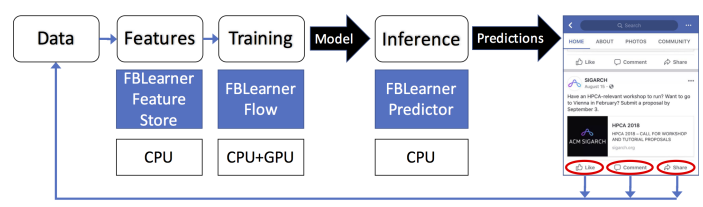
\includegraphics[width=80mm]{./imgs/grafico3.png}
\caption{Figura 1 -- Kit de ferramentas de Aprendizado de Máquina do Facebook}
%\end{minipage}
 \end{figure}

Fonte: Facebook\footnote{https://research.fb.com/wp-content/uploads/2017/12/hpca-2018-facebook.pdf}

Esse kit consiste num conjunto de três ferramentas, onde cada uma
concentra-se em diferentes partes do Aprendizado de Máquina. Segue
descrição dessas ferramentas: 1) o ``\emph{FBLearner Feature Store}'' é
um catálogo de vários geradores de recursos (dados) que podem ser usados
para treinamento e previsão em tempo real. Ter esta lista de recursos é
o ponto de partida para que as equipes comecem a usar o \emph{Machine
Learning}, além de ajudar a melhorar os modelos existentes com novos
recursos. Os dados são obtidos por meio das interações (curtidas,
comentários, compartilhamentos, fotos) que os usuários disponibilizam no
Facebook; 2) o ``\emph{FBLearner Flow''} funciona como um sistema de
gerenciamento que executa um fluxo de trabalho descrevendo as etapas
para treinar e/ou avaliar um modelo e os recursos (dados) necessários
para o seu uso. Possui ferramentas para o gerenciamento de experimentos
e uma interface com o usuário que controla todos os artefatos e métricas
gerados por cada execução ou experimento de fluxo de trabalho e 3) o
``\emph{FBLearner Predictor}'' é o mecanismo de inferência interna que
usa os modelos treinados no ``\emph{Flow}'' para fornecer previsões em
tempo real. O ``\emph{Predictor}'' é usado por várias equipes de
produtos no Facebook (Hazelwood et al, 2018, online).

Segundo Biddle (2018), o Facebook foi questionado a respeito do
``\emph{FBLearner Flow}'' e de quais dados dos usuários são usados para
prever comportamentos, ou se essa tecnologia poderia ser usada em outros
contextos mais sensíveis, como campanhas políticas ou assistência
médica. Em resposta, a equipe de relações públicas, do Facebook, afirmou
apenas que o ``\emph{FBLearner Flow} é utilizado para gerenciar fluxos
de trabalho e que o mesmo não é usado como um serviço de marketing.

É difícil comprovar se o Facebook utiliza o ``\emph{FBLearner Flow}''
para realizar previsões futuras dos usuários ou que tenha desenvolvido
alguma outra ferramenta com esta finalidade. No entanto, ao analisar a
patente ``\emph{Predicting Life Changes of Members of a Social
Networking System}\footnote{https://patents.google.com/patent/US20120016817A1/en}'',
registrada em 2010, fica claro o intuito dessa empresa em utilizar
Aprendizado de Máquina e \emph{Big Data} para prever ou inferir mudanças
futuras na vida dos usuários, como ``alteração do estado civil'',
``novos empregos'', ``nascimentos de filhos'', entre outras mudanças
significativas.

Na visão de Frank Pasquale, professor de Direito da Universidade de
Maryland e pesquisador sobre ética dos algoritmos da Universidade de
Yale, este projeto de previsão comportamental do Facebook é
``assustador''. Ele está preocupado com a possibilidade de que as
previsões do algoritmo sejam transformadas pela empresa em profecias
autorrealizáveis. ``Porque, uma vez feita a previsão, a empresa tem um
interesse financeiro na sua realização'' (Pasquale apud Biddle, 2018,
online).

De acordo com Jonathan Albright, diretor de Pesquisa do Tow Center for
Digital Journalism, da Universidade de Columbia, a segmentação de
anúncios via Aprendizado de Máquina ``sempre pode virar uma arma'' para
influenciar, por exemplo, a política. Ele se preocupa com os possíveis
usos dessas técnicas nas eleições (Albright apud Biddle, 2018, online).
Para Biddle (2018), os estímulos gerados pelo Aprendizado de Máquina já
são problemáticos quando se trata de incentivar uma compra, imagina o
quanto isso pode ser ao usar a tecnologia para angariar votos.

De acordo com Domingos (2017), ``foi o \emph{Machine Learning} que
elegeu'' Barack Obama em 2012. Segundo ele, a campanha de Mitt Rommey
seguiu uma ``abordagem convencional de consulta'', compilando os
eleitores em categorias genéricas. Já Obama, contratou Rayid Ghani,
especialista em \emph{Machine Learning}, para ser cientista-chefe de sua
campanha (Domingos, 2017, 40-41).

Rayid Ghani empreendeu a uma das ``maiores operações de análise da
história política". Ele reuniu todas as informações sobre eleitores em
um único banco de dados; cruzou estes dados com o que conseguiu minerar
em redes sociais, marketing e outras fontes; e com a análise de todos
esses dados conseguiu prever esses quatro itens para cada eleitor:
``qual a probabilidade de apoiar Obama; comparecer às pesquisas; reagir
aos lembretes da campanha e mudar de opinião a partir de uma troca de
ideias sobre um assunto especifico''. Com base nesse modelo, a campanha
realizou 66.000 simulações da eleição e de acordo com os resultados
direcionou as equipes com ``as informações de quem deveriam chamar, em
quais portas deveriam bater e o que dizer'' (Domingos, 2017, 41).

\begin{quote}
Na política, como nos negócios e na guerra, não há nada pior que ver seu
oponente realizar movimentos que você não entende e sobre os quais não
sabe o que fazer até ser tarde demais. Foi isso que aconteceu na
campanha de Romney. Eles podiam ver o adversário comprando anúncios em
determinadas emissoras a cabo de cidades especificas, mas não sabiam o
porquê; sua bola de cristal estava muito embaçada. No fim das contas,
Obama ganhou a preferência de todos os estados decisivos, exceto
Carolina do Norte, com margens maiores que o previsto até pelos mais
confiáveis peritos em opinião pública (Domingos, 2017, 41).
\end{quote}

Nas eleições de 2016, dos Estados Unidos, o uso de \emph{Machine
Learning} e \emph{Big Data} já não eram o que havia de mais moderno e
eficiente. Steve Bannon, conselheiro da campanha de Donald Trump e
membro do conselho da Cambridge Analytica, apresentou um novo arsenal
tecnológico muito mais potente. Para tal empreitada, a Cambridge
Analytica recebeu um investimento de US \$ 15 milhões de Robert Mercer,
bilionário cientista da computação americano, especializado em
Inteligência Artificial (Matthew et al, 2018). A meta era criar
ferramentas que pudessem identificar as personalidades dos eleitores
americanos e influenciar seu comportamento. A motivação veio de um
artigo de 2014, elaborado pelo Cambridge's Psychometrics Center,
denominado: ``\emph{Computer-based personality judgments are more
accurate than those made byhumans}'' (Youyou et al, 2014). Contudo, eles
ainda não tinham os dados necessários para tal empreitada (Matthew et
al, 2018).

De acordo com Matthew et al (2018), essa história começou quando
Alexander Nix, líder da divisão de eleições do \emph{SCL Group},
contratou Christopher Wylie com o objetivo de entrar no mundo de dados
políticos. Wylie foi ligado aos veteranos das campanhas do presidente
Obama e estava interessado em usar traços psicológicos para influenciar
o comportamento dos eleitores. Wylie encontrou a solução para criação da
nova ferramenta, no Centro de Psicometria, da Universidade de Cambridge.
Os cientistas dessa universidade desenvolveram uma técnica para mapear
traços de personalidade com base no que as pessoas curtiam no Facebook e
demais plataformas digitais. Para realizar esse estudo, os
pesquisadores, Michal Kosinski e seus colaboradores, criaram o
aplicativo \emph{MyPersonality}¸ conforme descrito anteriormente.

Segundo Matthew et al (2018), o Centro de Psicometria não aceitou a
proposta para trabalhar com a Cambridge Analytica. Wylie, então
encontrou o Dr. Kogan, professor de psicologia e especialista em
psicometria de mídias sociais, na Universidade de Cambridge, que
construiu seu próprio aplicativo, chamado "\emph{This is your Digital
Life}" e em junho de 2014 começou a coletar os dados para a Cambridge
Analytica.

Os usuários receberam um pagamento para baixar o aplicativo e conceder
suas informações do Facebook em troca do resultado do teste. Na época,
foram informados que esses dados seriam utilizados para fins acadêmicos.
O que não foi informado é que, além dos dados dos usuários, o aplicativo
também coletaria dados de toda a rede de amigos desses usuários e que
todos esses dados seriam utilizados para fins políticos.

De acordo com Matthew et al (2018), o aplicativo forneceu mais de 50
milhões de perfis brutos para a empresa. Desses perfis, cerca de 30
milhões continham informações que a empresa poderia construir perfis
psicográficos e apenas cerca de 270.000 usuários consentiram em ter seus
dados colhidos que foram aqueles que participaram da pesquisa.

Em síntese, a \emph{Global Science Research - GSR}, empresa de análise
de dados de Aleksandr Kogan em parceria com a Cambrigde Analytica que
foi financiada por um especialista em Inteligência Artificial, coletou
dados dos perfis do Facebook de milhões de eleitores americanos para
usá-los na construção de um algoritmo para prever e influenciar as
escolhas dos eleitores (Cadwalladr e Graham-Harrison, 2018).

Toda essa situação gerou uma grande indignação e culminou com a
Cambridge Analytica e o Facebook sendo focos de um inquérito sobre dados
e política feito pelo \emph{British Information Commissioner's Office},
uma autoridade independente, no Reino Unido que promove a proteção dos
dados pessoais\emph{.} De acordo com Cadwalladr e Graham-Harrison
(2018), o senador democrata, Mark Warner, disse que a coleta de dados em
uma escala tão ampla como essa para a segmentação política requer
controles mais rígidos e uma regulamentação da propaganda política
on-line da mesma forma que a televisão, o rádio e a mídia impressa.

\section{Considerações Finais}

Os resultados das pesquisas com base em psicometria, rastros digitais
dos usuários e Aprendizado de Máquina mostraram que: julgamentos de
personalidade feitos por algoritmos são mais precisos do que os
realizados por humanos e a persuasão digital em massa é eficaz quando se
tem um grande volume de dados e é feita uma análise minuciosa e com alta
precisão para segmentação e direcionamento de mensagens personalizadas.

As eleições de Barack Obama, em 2012 e Donald Trump, em 2016, são
exemplos do mundo real (fora da academia e do laboratório) de utilização
do Aprendizado de Máquina como dispositivo de modulação para fins
políticos.

No entanto, a predição do comportamento dos eleitores, nas eleições
americanas de 2016, para segmentação e direcionamento de discurso
político personalizado, gerou vários questionamentos. Em 2018, quando o
escândalo da Cambridge Analytica e o vazamento de dados dos usuários do
Facebook vieram à tona, esses questionamentos ganharam força e acendeu
um alerta para a privacidade dos dados pessoais e a necessidade de uma
regulamentação da propaganda política on-line entre outras medidas.

Diante de tudo isso, ficam as seguintes perguntas: ``Todo esse
maquinismo abre possibilidades e potencialidades para emancipação ou
eles conduzem de modo inelutável à catástrofe'' (Lazzarato, 2014,39)?
``Da privacidade ao futuro do trabalho e à ética da guerra robotizada,
veremos onde estão os problemas e como resolvê-los'' (Domingos, 2017,
22)?

Obter as respostas e ações efetivas para estes questionamentos é uma
tarefa árdua. Um caminho possível requer como primeiro passo um
exaustivo trabalho de conscientização das pessoas. É preciso que elas
saibam o valor de cada curtida, post e comentário e o quanto isso revela
sobre suas vidas e principalmente a influência que isso implica nas suas
escolhas diárias, desde o ato de votar até a simples compra de um livro
e como isso pode ser monetizado pelas plataformas digitais. Concluído o
primeiro passo, vem a parte mais difícil que é definir uma
regulamentação que permita a governança desses algoritmos e a
privacidade dos dados.

\section{Referências}

AMORIM, Paula Fernanda Patrícia de. \textbf{A crítica de John Searle à
Inteligência Artificial: Uma abordagem em filosofia e mente}.
2014. 99f. Dissertação (Mestrado em Filosofia) -- Universidade Federal
da Paraíba, PB.

BIDDLE, Sam. \textbf{Facebook usa inteligência artificial para prever o
comportamento de usuário para anunciantes}. Tradução: Tradução: Bernardo
Tonasse. 2018. The Intercept\_Brasil. Disponível em:
\textless{}https://theintercept.com/2018/04/13/facebook-inteligencia-artificial/\textgreater{}.
Acesso em: 08 jun. 2018.

BORINI, Guilherme. \textbf{Facebook investe US\$ 30 milhões para
aquisição de startup de inteligência artificial}. 2018. Disponível em:
\textless{}https://computerworld.com.br/2018/0
7/05/facebook-investe-us-30-milhoes-para-aquisicao-de-startup-de-inteligencia-artificial/\textgreater{}.
Acesso em : 27 set. 2018.

CADWALLADR, Carole. \textbf{The Cambridge Analytica Files - `I made
Steve Bannon's psychological warfare tool': meet the data war
whistleblower}. 2018. Disponível em:
\textless{}https://www.theguardian.com/news/2018/mar/17/data-war-whistleblower-christopher-wylie-faceook-nix-bannon-trump\textgreater{}.
Acesso em: 11 jun. 2018.

CADWALLADR, Carole e GRAHAM-HARRISON, Emma. \textbf{Revealed: 50 million
Facebook profiles harvested for Cambridge Analytica in major data
breach}. 2018. Disponível em:
\textless{}https://www.theguardian.com/news/2018/mar/17/
cambridge-analytica-facebook-influence-us-election\textgreater{}.
Acesso em: 11 jun. 2018.

CAVALHEIRO, Glauco e BRANDÃO, Carolina Gandon. Ensaio 3, ``Comunicação e
retórica: Um contexto teórico para pensar a pós-verdade''. In:
GUARESCHI, Pedrinho A; AMON, Denise e GUERRA, André. \textbf{Psicologia,
Comunicação e Pós-verdade}. Porto Alegre: Abrapso, 2017. P. 83-100.

DELEUZE, Gilles. \textbf{Conversações}. São Paulo: Editora 34. 1992.

DOMINGOS, Pedro. \textbf{O algoritmo mestre}. São Paulo: Novatec. 2017.

FOUCAULT, Michel. \textbf{Microfísica do Poder}. Rio de Janeiro: Paz \&
Terra, 2015.

GUARESCHI, Pedrinho. Ensaio 5 -- ``Psicologia e Pós-Verdade''. In:
GUARESCHI, Pedrinho A; AMON, Denise e GUERRA, André. \textbf{Psicologia,
Comunicação e Pós-verdade}. Porto Alegre: Abrapso, 2017. P. 161-193.

HAAS, Guilherme. \textbf{Google compra DeepMind, startup de programação
em inteligência artificial}. 2014. Disponível em:
\textless{}https://www.tecmundo.com.br/google/4960
8-google-compra-deepmind-startup-de-programacao-em-inteli
gencia-artificial.htm\textgreater{}.
Acesso em: 27 set. 2018.

HAZELWOOD, Kim, et al. \textbf{Applied Machine Learning at Facebook: A
Datacenter Infrastructure Perspective}\emph{.} 2018. Disponível em:
\textless{}https://research.fb.com/publications/
applied-machine-learning-at-facebook-a-datacenter-infrastru
cture-perspective/\textgreater{}.
Acesso em: 07 jun. 2018.

JÚNIOR, Gilberto Timótheo e LIMA, Sérgio Muinhos Barroso.
\textbf{Algoritmos Genéticos Aplicados a Jogos Eletrônicos}. Revista
Eletrônica da Faculdade Metodista Granbery, Curso de Sistemas de
Informação - N. 8. 2010. Disponível em:
\textless{}http://re.granbery.edu.br/artigos/MzU2\textgreater{}. Acesso
em: 28 set. 2018.

KOSINSKI, Michal, STILLWELLA, David, e GRAEPELB, Thore.
\emph{\textbf{Private traits and attributes are predictable from digital
records of human behavior}}. PNAS, vol. 110, no. 15, 9 abr. 2013.
Disponível em:
\textless{}http://www.pnas.org/content/pnas/110/
15/5802.full.pdf\textgreater{}.
Acesso em 05 jun. 2018.

KOSINSKI, Michal, WANG, Yilun, LAKKARAJU, Himabindu e LESKOVEC, Jure.
\textbf{Mining Big Data to Extract Patterns and Predict Real-Life
Outcomes}. Psychological Methods, Vol. 21, No. 4, 2016. Disponível em:
\textless{}http://www.apa.org/pubs/journals/features/met-met0000104.pdf\textgreater{}.
Acesso em: 05 jun. 2018.

LAZZARATO, Maurizio. \textbf{As revoluções do capitalismo.} Rio de
Janeiro: Civilização Brasileira, 2006.

LAZZARATO, Maurizio. \textbf{Signos, Máquinas, Subjetividades.} São
Paulo: Edições Sesc, 2014.

MATTHEW, Rosenberg et al. \textbf{How Trump Consultants Exploited the
Facebook Data of Millions.} 2018. Disponível em:
\textless{}https://www.nytimes.com/2018/03/17/us/politics/cam
bridge-analytica-trump-campaign.html\textgreater{}.
Acesso em: 11 jun. 2018.

MATZA, C, KOSINSKI, M. NAVEC, G. e STILLWELLD, D. J.
\textbf{Psychological Targeting as an Effective Approach to Digital Mass
Persuasion}. PNAS, vol. 114, no. 48, 28 nov. 2017. Disponível em:
\textless{}http://www.pnas.org/content/pnas/114/48/12
714.full.pdf\textgreater{}.
Acesso em: 05 jun. 2018.

MCCULLOCH, Warren S. e PITTS, Walter. \textbf{A logical calculus of the
ideas immanent in nervous activity}. Bulletin of Mathematical
Biophysics, Volume 5. 1943. Disponível em:
\textless{}https://pdfs.semanticscholar.org/5272/8a99829792c327
2043842455f3a110e841b1.pdf
\textgreater{}. Acesso em: 28 set. 2018.

MOREIRA, Daniel. \textbf{O que é uma startup?} 2018. Disponível em:
\textless{}https://exame.abril.com.br/pme/o-que-e-uma-startup/\textgreater{}.
Acesso em: 16 jul. 2018

PRAUDE, Carlos Correia. \textbf{Arte Computacional e Teoria Ator-Rede:
actantes e associações intersubjetivas em cena}. Tese (Tese em Arte) -
Universidade de Brasília. Brasília. 2015.

SEARLE, John R. \textbf{Minds, brains, and programs.} The Behavioral and
Brain Sciences. v. 3, p. 417-457. Cambridge University Press. 1980.
Disponível em:
\textless{}http://cogprints.org/
7150/1/10.1.1.83.5248.pdf\textgreater{}.
Acesso em: 17 jul. 2018.

SILVEIRA, Sergio Amadeu da. \textbf{Tudo sobre todos. Redes digitais,
privacidade e venda de dados pessoais}. São Paulo: Edições Sesc, 2017.

SUGOMORI, Yusuke. \textbf{Java Deep Learning Essentials.} Packt
Publishing: Birmingham. 2016.

TURING, A. M. \textbf{Computing Machinery and Intelligence}. Mind, v.
59, no. 236, p. 433-460, out. 1950. Disponível em:
\textless{}https://www.csee.umbc.edu/courses/471/papers/turi
ng.pdf\textgreater{}
Acesso em: 21 mai. 2018.

VINGE, Vernor. \textbf{The coming technological singularity: How to
survive in the post-human era}. Interdisciplinary Science and
Engineering in the Era of Cyberspace, v. 10129, oNASA Conference
Publication, p. 11---22, Cleveland, OH, NASA Lewis Research Center,
1993. Disponível em:
\textless{}https://ntrs.nasa.gov/search.jsp?R=19940022856\textgreater{}
Acesso em: 29 mai. 2018.

YOUYOU, Wu, KOSINSKIB, Michal e STILLWELLA, David.
\textbf{Computer-based personality judgments are more accurate than
those made by humans.} PNAS, v. 112, no. 4, 27 jan. 2014. Disponível em:
\textless{}http://www.richardbenjamintru
st.co.uk/uploads/finalreports/2013/DStillwell.pdf\textgreater{}
Acesso em: 11 jun. 2018.
